\graphicspath{{./figs/repo/}{./figs/}}
\section{Optical Proximity Correction (OPC)}

%zhaowenqian

\begin{frame}{What is Reinforcement Learning:}
    
    \begin{itemize}
        \item different from either supervised or unsupervised learning\\

        \begin{center}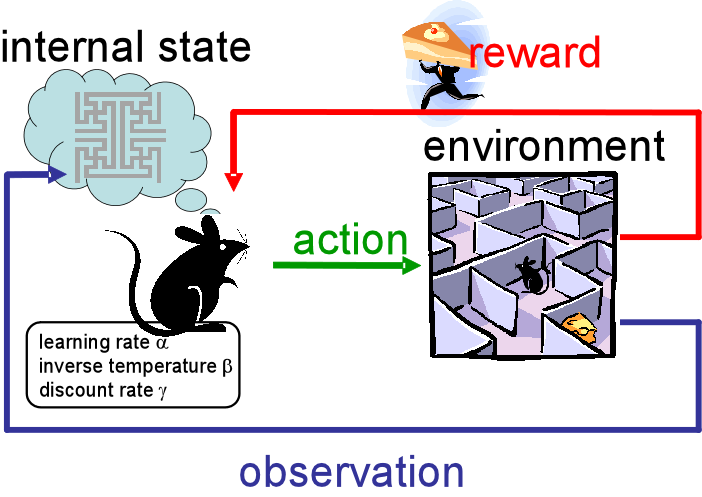
\includegraphics[width=.6\textwidth]{rl_intro}\end{center}
   
        
    \end{itemize}
\end{frame}


\begin{frame}{What is Reinforcement Learning:}
    
    \begin{itemize}
        \item Background\\

        \begin{center}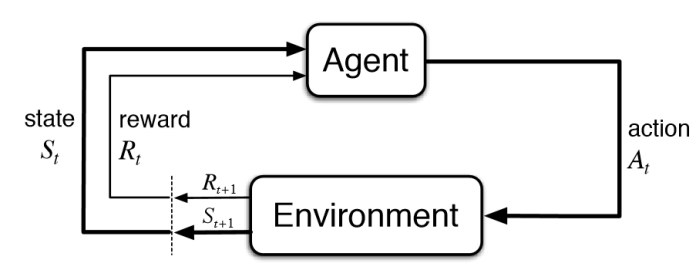
\includegraphics[width=.4\textwidth]{rl_intro2}\end{center}
        \hspace{0.5cm}$\bullet$ Agent: take actions\\
        \hspace{0.5cm}$\bullet$ Action: S set of possible moves that Agent can make\\
        \hspace{0.5cm}$\bullet$ Environment: input: state and action taken, output: reward\\
        \hspace{0.5cm}$\bullet$ Policy: the strategy for agent to take actions\\
        \hspace{0.5cm}$\bullet$ Discount factor: dampen to make discounted future reward\\
        \hspace{0.5cm}$\bullet$ goal: obtain strategy to optimize:
        \begin{equation}
         \sum_{t=0}^{t=\infty} \gamma_{t}r(x(t),a(t))
        \end{equation}


   
        
    \end{itemize}
\end{frame}

\begin{frame}{Markov Decision Process}
    \begin{itemize}
        
        \item The MDP gives us a precise formulation of the environment, given a state st we select an action $a_{t}$ and observe $s_{t+1}$ and $r_{t}$ according to the transition probabilities P:\\
        \bigskip
        \hspace{0.5cm}$\bullet$  $S$ - set of possible states \\
        \hspace{0.5cm}$\bullet$  $s_{t}\in S$ - state at step $t$ \\
        \hspace{0.5cm}$\bullet$  $A$ - set of possible actions \\
        \hspace{0.5cm}$\bullet$  $a_{t}\in A$ - selected action at step $t$\\
        \hspace{0.5cm}$\bullet$  $R$ - Reward function. The reward at step $t$ is given by $r_{t+1} = R(s_{t}, a_{t}, s_{t+1})$\\
        \hspace{0.5cm}$\bullet$ $P$ - transition probabilities such that $s_{t+1} \sim P(s|s_{t},a_{t})$, i.e. \\
        \hspace{0.5cm}$\bullet$  $\rho$ - Initial state distribution such that $s_{0} \sim \rho(s)$\\
        \bigskip
        \item Agent is defined with a policy function $\pi(a|s)$, mapping from states to actions and can be either deterministic or non-deterministic
        
    \end{itemize}
\end{frame}

\begin{frame}{Markov Decision Process}
    \begin{itemize}
        \item Given an MDP and a policy, an episode can be produced by repeating of:\\

        \hspace{0.5cm}$\bullet$  $a_{t} ∼ \pi(a|s_{t})$\\
        \hspace{0.5cm}$\bullet$  $s_{t+1} ∼P(s|s_{t},a_{t})$ \\
        \hspace{0.5cm}$\bullet$  $r_{t+1} =r(s_{t},a_{t},s_{t+1})$ \\  
        \item which produce:\\
            \begin{center}
                episode $:= s_{0},a_{0},r_{1},s_{1},a_{1},r_{1},...,s_{\tau−1},a_{\tau−1},r_{\tau−1},s_{\tau}$
            \end{center}
        \bigskip
        \item Optimal Solution gives: \\
            \begin{equation}
                \max\limits_{\pi} E [\sum_{t=1}^{\tau} r_{t}]
            \end{equation}
        
    \end{itemize}
\end{frame}


\begin{frame}{Markov Decision Process}
    \begin{itemize}
        \item Value function defined as :
            \begin{equation}
                V^{\pi}(s)=E_{\pi} [\sum_{t=1}^{\tau} r_{t}|s_{0}=s]
            \end{equation}
            \begin{equation}
                V^*(s)=\max\limits_{\pi} E_{\pi} [\sum_{t=1}^{\tau} r_{t}|s_{0}=s]
            \end{equation}
        \item Bellman equation: A recursive relation for value function:
            \begin{equation}
                V^*(s)=\max\limits_{a\in A} E [r_{t+1}+V^*(s_{t+1})|s_{t}=s,a_{t}=a]
            \end{equation}
        \item $(TV)(s)$ is the Bellman operator and we can recursively calculate it and update $V(s)$ (value iteration) to reach optimal (Monotonicity and Contraction mapping)
            \begin{equation}
                (TV)(s)=\max\limits_{a\in A} E [r_{t+1}+V^*_{s_{t+1}}|s_{t}=s,a_{t}=t]
            \end{equation}
            \begin{equation}
            V_{k+1}=TV_{k}
            \end{equation}
        \item policy iteration use the same idea, but instead of updating value function, it update Policy $\pi$

        
    \end{itemize}
\end{frame}


\begin{frame}{Markov Decision Process}
    \begin{itemize}
        \item Another approach: State-Action Value Function: define a quantity $Q: S \times A\rightarrow \mathbb{R}$:\\
        \begin{equation}
        Q^\pi(s,a)=\bar{R}(s,a)+\sum_{s' \in S}^{T} P_{s,a} (s')V^\pi(s')
        \end{equation}
        \item  Recursively Calculate optimal by using Bellman Operator:
        \bigskip
        
        \hspace{0.5cm}$\bullet$ $ FQ(s,a)=\bar{R}(s,a)+\sum_{s' \in S}^{T} P_{s,a} (s') \max\limits_{a'\in A} Q (s',a') $\\
        \hspace{0.5cm}$\bullet$  $Q(s,a)=FQ(s,a)$
        \bigskip
        
        \item Greedy action selection is simple:
        \begin{equation}
        \pi(s)=\arg\max\limits_{a \in A}Q(s_{t},a)
        \end{equation}
    \end{itemize}
\end{frame}


\begin{frame}{MDP vs RL}
    \begin{itemize}
        \item Difference between Markov Decision Process and Reinforcement learning:\\
        \bigskip
        \hspace{0.5cm}$\bullet$  MDP: the transition matrix $P(s'|s,a)$ is known $\rightarrow$ used to find the optimal agent\\
        \hspace{0.5cm}$\bullet$  RL: $P(s'|s,a)$ unknown and need to be learned :\\
        \hspace{1cm}\romannumeral1 . Iteracting with environment \\
        \hspace{1cm}\romannumeral2 . Requiring explicit knowledge of $P$
        \bigskip
        \item But the same idea of state-action value function can be used for Reinforcement learning
        
    \end{itemize}
\end{frame}

\begin{frame}{Q-learning and SARSA}
    \begin{itemize}
        \item Q-learning:\\
        \bigskip
        \hspace{0.5cm}\romannumeral1 .  Build a Q-table which stores $Q(s,a)$ for each $s$ and $a$ (randomly initialized). i.e.\\
        \begin{center}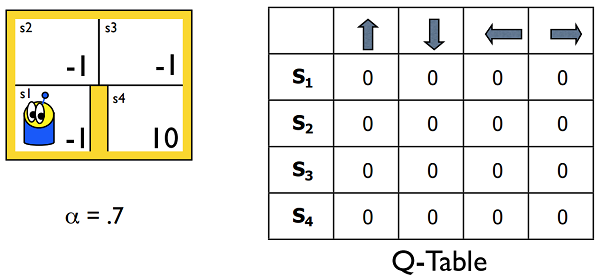
\includegraphics[width=.6\textwidth]{q_table}\end{center}
        
    \end{itemize}
\end{frame}

\begin{frame}{Q-learning and SARSA}
    \begin{itemize}
        \item Q-learning:\\
        \bigskip
        \hspace{0.5cm}\romannumeral2 . update $Q(s,a)$ with:\\
        \begin{equation}
            Q_{k+1}:=(1-\gamma_{k})Q_{k}+\gamma_{k}(r+\max\limits_{a' \in A}Q_{k}(s',a'))
        \end{equation}
        \hspace{0.7cm} where $\gamma_{k}$ is the learning rate, with $\sum_{k=1}^{\infty}\gamma_{k}=\infty$ and $\sum_{k=1}^{\infty}\gamma^2_{k}<\infty $ :\\
        \begin{equation}
            Q_{k+1}=Q_{k}+\gamma_{k}(r+\max\limits_{a' \in A}Q_{k}(s',a')-Q_{k}(s,a))
        \end{equation}
        \item Q-learning Demo: \href{https://youtu.be/imKK9bpGlaQ}{maze 4*4} \\
        
    \end{itemize}
\end{frame}

\begin{frame}{Q-learning and SARSA}
    \begin{itemize}
        \item Q-learning result:\\
        \begin{center}Reward of episodes of experiment on Maze game 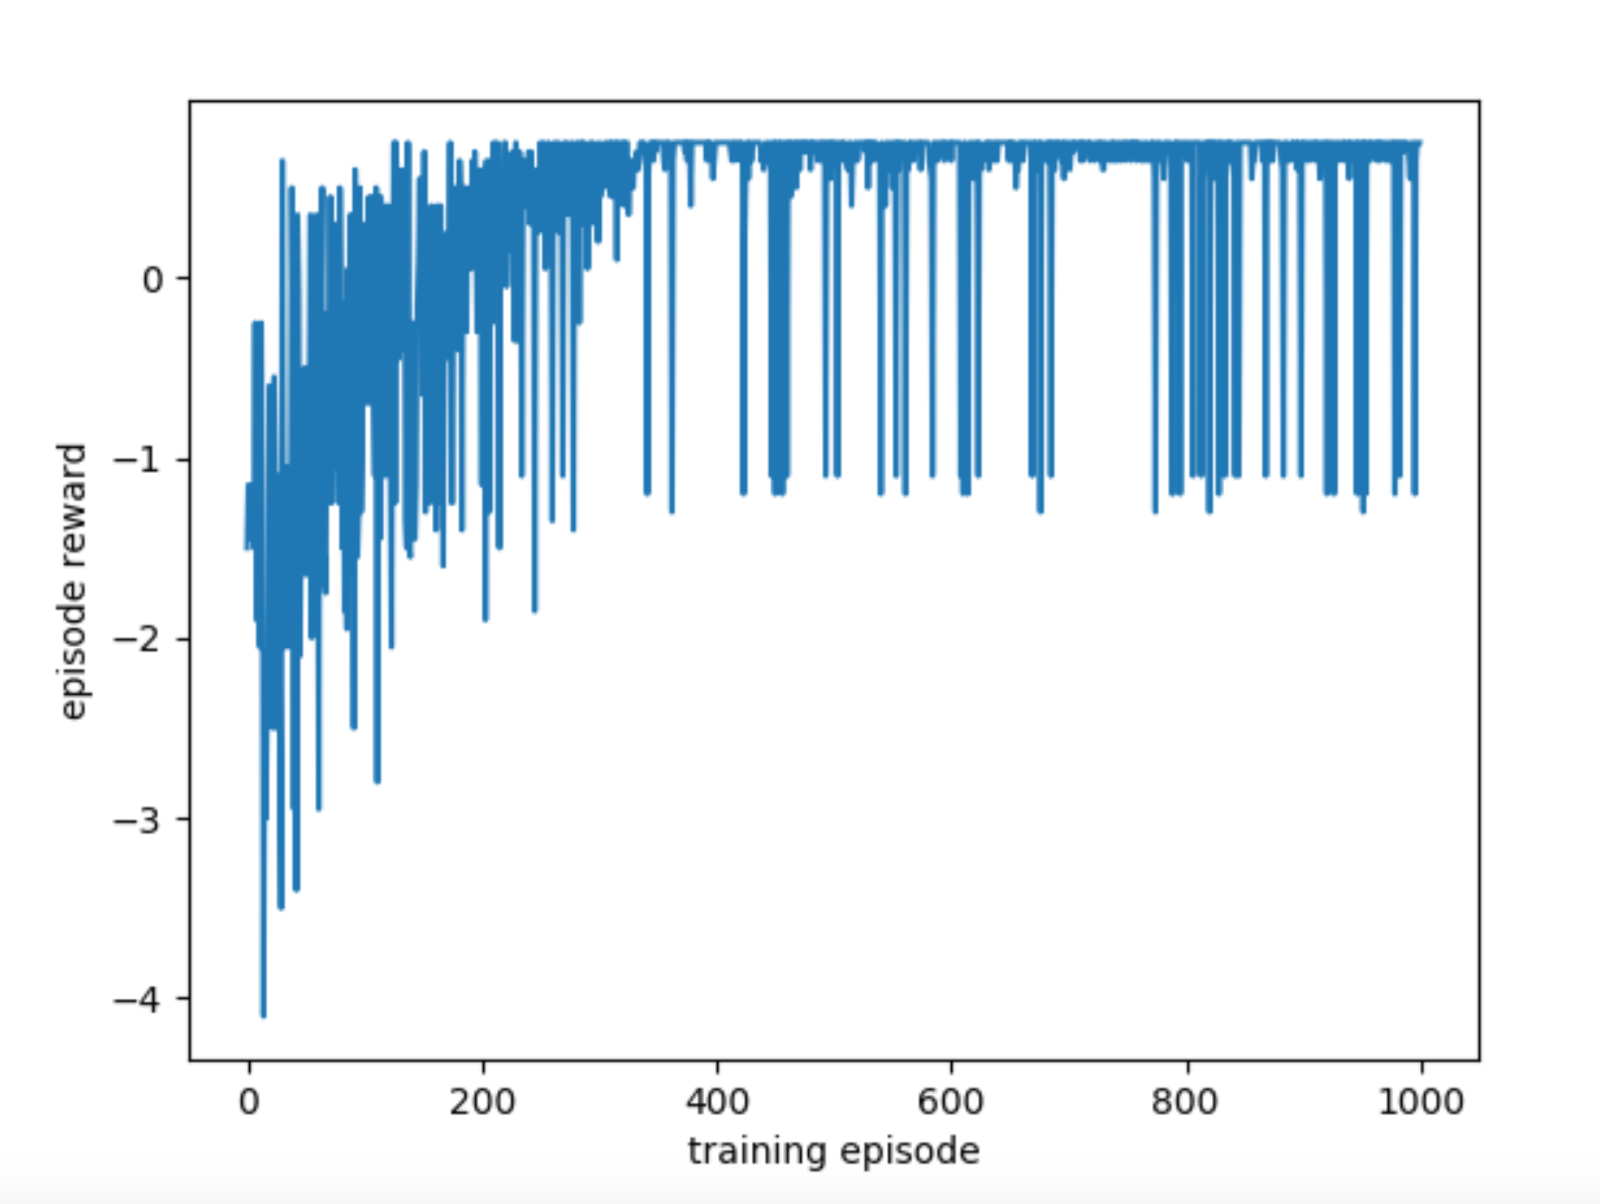
\includegraphics[width=0.6\textwidth]{q_learning_result}\end{center}

    \end{itemize}
\end{frame}

\begin{frame}{Q-learning and SARSA}
    \begin{itemize}
        \item Exploration: $\epsilon - greedy$\\
        \begin{equation}
            a_{t}=\begin{cases}
             \arg\max_{a \in A}Q_{s_{t},a}, & \text{w.p.   } 1-\epsilon.\\
             unif(A), & \text{w.p.   } \epsilon.
        \end{cases}
        \end{equation}

        \item SARSA:\\
        \hspace{0.5cm}$\bullet$  update based on the current play $(s,a,r,s',a')$ \\
        \begin{equation}
            Q_{k+1}=Q_{k}+\gamma_{k}(r+Q_{k}(s',a')-Q_{k}(s,a))
        \end{equation}
        \hspace{0.5cm}$\bullet$  Similar to Q-learning but is On-policy \\


    \end{itemize}
\end{frame}



\begin{frame}{Deep Q-Networks}
    \begin{itemize}
         \item Drawback of Q-learning and SARSA:\\
         \bigskip
         \hspace{0.5cm}$\bullet$ Q-table can be too big if environment is complicate i.e. $10^6\times10^3$ maze\\
         \bigskip
         \item Alternative Algorithm: DQN:\\
         \bigskip
         \hspace{0.5cm}$\bullet$ Use a function approximator to estimate action-value function with Q-Network\\
         \bigskip
         \item Steps:\\
         \bigskip
         \hspace{0.5cm}$\bullet$ store transition$(s_{t},a_{t},r_{t+1},s_{t+1})$ in memory\\
         \hspace{0.5cm}$\bullet$ sample mini-batch of transitions, optimise MSE between Q-network and \\
         \hspace{0.7cm} Q-learning targets:\\
         \begin{equation}
            \text{minimize  }  L_{w}=E_{s,a,r,s'}[(r+\gamma \max\limits_{a'}Q(s',a';w^{-})-Q(s,a;w))^2]
        \end{equation}
        \hspace{0.5cm}$\bullet$ Important tricks: experience replay and fixed target

    \end{itemize}
\end{frame}


\begin{frame}{Deep Q-Networks(DQN): play games in OpenAI gym}
    %{{{
    \begin{center}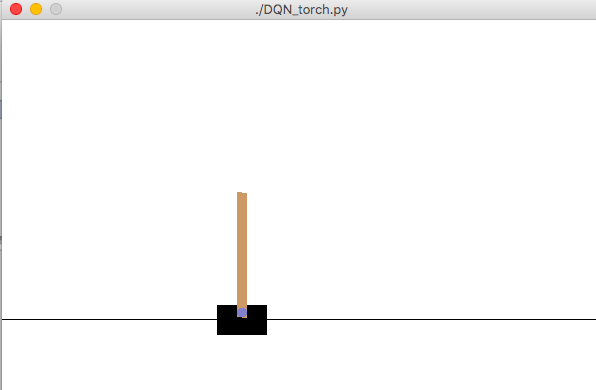
\includegraphics[width=.4\textwidth]{pole}\end{center}
    \begin{itemize}
        \item States are represented by 4-element tuples (position,cart velocity,angle,tip velocity)
        \item Actions can be either moving left or right
        \item Function approximator is a feed foward neural network 
        \item 1 hidden layer with 10 neurons, 2 output neurons representing value estimation for two actions
        \item Implemented using torch and tensorflow, can stay alive for 1 minute
    \end{itemize}

\end{frame}







